
\section{Project Tango} \label{sec:theory_project_tango}

Project Tango ist eine Technologie Plattform für Android Tablets und Smartphones von Google’s Advanced Technology and Projects Group (ATAP). Das Ziel dieser Plattform ist es Motion Tracking (Positionierung), Depth Perception (Tiefeninformation/Pointcloud) und Area Learning (Lokalisierung) auf mobile Endgeräte zu bringen, um verschiedenste Anwendungs-Szenarien abzudecken. Typische Szenarien sind Indoor Navigation, Virtual Reality Anwendungen, Vermessungs- und Rekonstruktions Software und Augmented Reality Anwendungen.

Das System ermöglicht in erster Linie ein Tracking von Positionsänderungen des Geräts im Raum und bietet somit eine genaue relative Lokalisierung. Mit Hilfe dieser Lokalisierung und der Hinzunahme von visuellen Merkmalen im Raum, ist das Gerät in der Lage, seine Umgebung kennenzulernen und gegebenenfalls die Lokalisierung zu korrigieren oder aber Diese in einer bereits erlernten Umgebung zu bestimmen. Zusätzlich bietet Project Tango die Möglichkeit, mit Hilfe eines Tiefensensors, eine Pointcloud der Tiefeninformation pro Bildausschnitt zu ermitteln, um Anwendungen auch räumliche Informationen bereitzustellen.  \citep{Proje19:online} 

\subsection{Geräte und Hardware}

Da das Project Tango zum Zeitpunkt der Verfassung dieser Thesis noch unter Entwicklung steht, gibt es von Google erste Entwickler Prototypen. Das Erste Gerät \enquote{Peanut Phone} im Smartphone Format, welches in Abbildung \ref{fig:tango-device} rechts unten zu erkennen ist, wurde Anfang 2014 veröffentlicht und ein halbes Jahr später bereits durch eine neue Generation, dem \enquote{Yellowstone Tablet} ersetzt. Dieses 7\dq Tablet, zu sehen rechts oben im Bild \ref{fig:tango-device}, verfügt, wie in der Abbildung links zu erkennen, über einen Infrarot Laser Projektor, eine Fisheye Kamera und eine normale 4 Megapixel Kamera auf der Rückseite. Zudem sind, wie in aktuellen Smartphones und Tables üblich, ein Beschleunigungssensor, Umgebungslichtsensor, Barometer, Kompass, GPS und ein Gyroskop verbaut. Das Gerät wird von einem NVIDIA Tegra K1 Prozessor betrieben und verfügt über 4GB Arbeitsspeicher. \citep{Proje19:online} Mit diesem Gerät wurden die später beschriebenen Techniken umgesetzt und evaluiert. 

\begin{figure}[h]
  \centering
	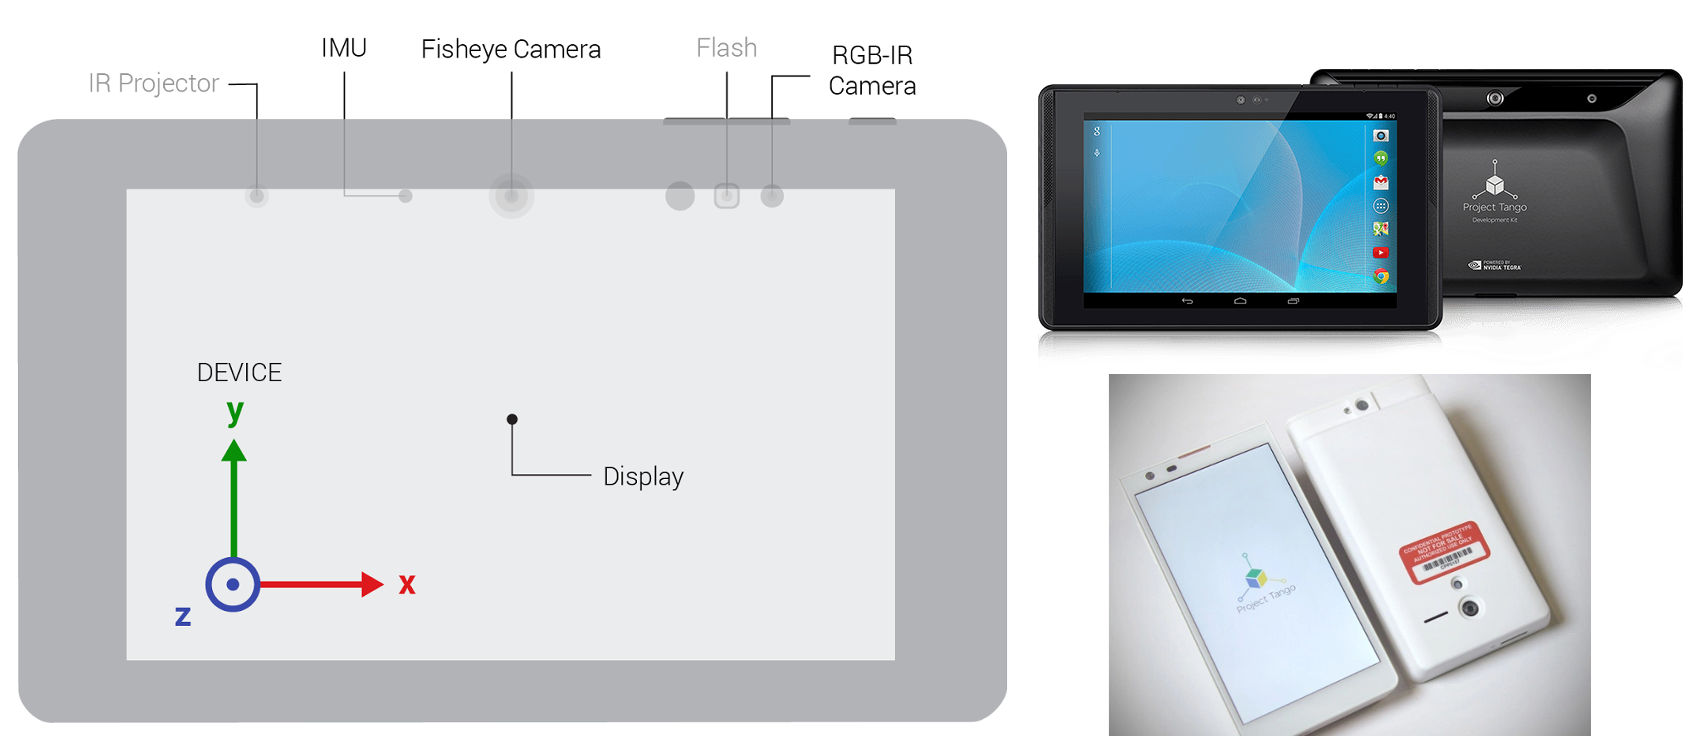
\includegraphics[width=1.0\textwidth]{content/images/theory/tango-device.png} 
  \caption{Links: schematischer Aufbau der Google Project Tango Hardware. Rechts: Das aktuelle Entwickler Gerät im Tablet Format (oben) und das alte Entwickler Gerät im Smartphone Format (unten). Übernommen von \citet{GoogleDevelopers:online}}
  \label{fig:tango-device}
\end{figure}

\subsection{Konzepte und Schnittstellen}

Generell betrachtet ist das Project Tango eine Plattform, die Computer Vision nutzt, um dem Gerät die Möglichkeit bietet seine relative Positionierung in der umgebenen Szene Echtzeit zu bestimmen. Auf den Geräten kommt Googles Android Betriebsystem zum Einsatz, weshalb zu beachten ist, dass es sich bei der Platform nur bedingt um eine Echtzeit Umgebung handelt. Das liegt daran, dass der Linux Kernel keine Garantien für die zeitlich präzise Ausführung von Instruktionen auf Grund von Scheduling geben kann. Google weist daher darauf hin, dass das System als \enquote{soft-realtime} betrachtet werden sollte. Daher sollten Messergebnisse verschiedener Sensoren unter Berücksichtigung ihrer Aufnahme Zeitpunkte verwendet werden. \citep{GoogleDevelopersConcepts:online} 

\subsubsection{Motion Tracking}

Um die relative Bewegung vom Start des Project Tango Systems bestimmen zu können nutzt es \enquote{visual-inertial odometry}. \citep{GoogleDevelopersConcepts:online}
Dabei handelt es sich um eine erweiterte Variante von Visual Odometry. 
Das von \citet{nister2004visual} veröffentlichte Verfahren Visual Odometry ist in der Lage aus einfachen Video Inhalten in Echtzeit die Bewegung der Kamera zu bestimmen. 
Hierzu werden zunächst übergreifende Features, zum Beispiel Punkte aus der \citet{harris1988combined} Kantenerkennung, aus mehreren Bildern bestimmt. Um daraus eine Transformation zwischen den Bildern ermitteln zu können wird der 5-point Algorithmus von \citet{nister2004efficient} angewendet. Dieser Algorithmus ist in der Lage das Problem zu lösen, eine relative Transformation zwischen zwei Bildern mit gegebenen 5 Punktübereinstimmungen zu ermitteln. Außerdem wird erwähnt, dass mit Hilfe des Schätzverfahrens RANSAC (beschrieben in Absatz \ref{sec:ransac}) bei einer Überbestimmung des Modells, ein potentieller Fehler deutlich minimiert werden kann. 

Project Tango lässt an dieser Stelle die internen Sensoren zur Rotation, Orientierung und Bewegung mit in die Bestimmung der Kamera Transformation einfließen, um so ein akkurates Ergebnis erzielen zu können. Über eine längere Messzeit oder eine größere Entfernung vom Ursprung kann es jedoch zu kleinen Abweichungen kommen. Außerdem existiert zum aktullen Zeitpunkt noch ein \enquote{Drift} Problem, was zu großen Messfehlern führen kann. Es wird jedoch versucht diese Probleme mit dem Konzept \enquote{Area Learning}, beschrieben in Kapitel \ref{subsec:area-learning}, zu lösen. \citep{GoogleDevelopersConcepts:online}

Wie genau das Verfahren aussieht, welche Techniken zur Feature Detection oder Feature Matching genutzt wird und welche Features hierfür erkannt werden ist nicht bekannt. \citet{Klingensmith_2015_7924}, als Mitglieder Googles Advanced Technologies and Projects Abteilung ATAP, erwähnen jedoch, dass nähere Informationen über das Verfahren von \citet{kottas2013consistency} und \citet{mourikis2007multi} beschrieben werden. Sie erläutern in Ihren Arbeiten, welche Mechanismen eingesetzt werden können, um eine Migration aller Sensor Informationen für ein zuverlässiges hybrides optisches Tracking zu realisieren.

\subsubsection{Deph Perception}

Zur Tiefenmessung ist die Project Tango Hardware mit einem kalibrierten Infrarot Laser Projektor ausgestattet. Dieser streut Infrarot Punkte mit einer Auflösung von 320 x 180 Punkten in den Raum, um dann, mit Hilfe von Aufnahmen der RGB Kamera, eine Punktewolke der Tiefeninformation zu bestimmen. Auf Grund einer ausgewogenen Konfiguration zwischen Messbereich, Messfehlern und dem Energieverbrauch, liegt der Messbereich der Sensorkombination, laut \citet{GoogleDevelopersConcepts:online}, zwischen einem halben und vier Metern. 

Dadurch dass diese Technologie auf der Aufnahme von projiziertem Infrarot Licht basiert, ist ein Einsatz der Tiefenmessung außerhalb geschlossener Räume nicht möglich. \citep{GoogleDevelopersConcepts:online} Außerdem entstehen Messfehler durch reflektierende,  lichtabsorbierende oder zu komplex strukturierte Oberflächen, wie zum Beispiel Metalle, LCD Monitore oder Hochflor Teppiche. 

Die zuvor erwähnten Punktewolken werden in dem eigens definierten XYZij Format von der Entwicklungsschnittstelle zurück gegeben. Dabei wird jeder Punkt mit den \(X\),\(Y\) und \(Z\) Koordinaten im Weltkoordinatensystem und den beiden Indizes \(i \) und \(j \) für die Spalte und Zeile der projizierten Punkte auf der Bildebene angegeben \citep{GoogleDevelopersConcepts:online}. Man spricht dabei von einer organisierten Punktewolke, da durch die \(i\) und \(j\) Koordinaten die direkten Nachbarn, ausgehend von dem Aufnahmeblickwinkel, eines Punktes bestimmt werden können. Hieraus ist es möglich Tiefenbilder, die sogenannten \enquote{Depth Maps}, zu bestimmen, für die es viele verschiedene Computer Vision Verfahren zur Bestimmung von Objekten, Strukturen und Fluchtpunkten gibt. Die Schnittstellen liefern jedoch zum aktuellen Entwicklungsstand die beschriebenen Informationen über die Spalten \(i\) und Zeilen \(j\), laut \citet{GoogleDevelopersKnownIssues:online}, noch nicht.

\citet{GoogleDevelopersConcepts:online} weist darauf hin, dass das Generieren von Polygon basierten Rekonstruktionen noch nicht in den Schnittstellen enthalten sind. Es gibt jedoch freie Dritt-Bibliotheken und -Systeme, wie das Robot Operating System \footnote{\url{http://ros.org/} (23.02.2016)} oder die Point Cloud Library\footnote{\url{http://pointclouds.org/} (23.02.2016)}, die für eine weitere Verarbeitung genutzt werden können.

\subsubsection{Area Learning} \label{subsec:area-learning}

Area Learning bezeichnet den Prozess indem Project Tango Geräte in der Lage sind durch visuelle Hinweise die umgebenen Welt kennenzulernen und auf die Position des Gerätes zu schließen. 
Es ermöglicht somit eine Unterstützung für Motion Tracking und löst das Problem das Gerät in einer bereits bekannten Umgebung zu lokalisieren, wie in Abbildung \ref{fig:area-learning} links zu erkennen.
Project Tango bietet außerdem die Möglichkeit diese visuellen Hinweise und Ihre Position im Raum in sogenannten \enquote{Area Description Files} zu speichern und wiederzuverwenden. \citep{GoogleDevelopersConcepts:online}

\begin{figure}[h]
  \centering
	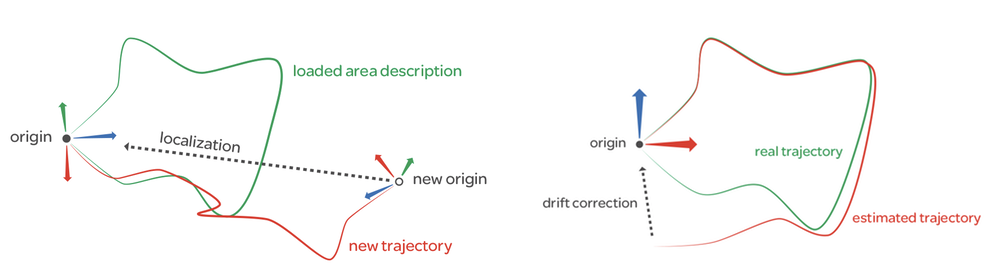
\includegraphics[width=1.0\textwidth]{content/images/theory/tango-area-learning.png} 
  \caption{Links: Lokalisierungsprozess durch Area Learning. Rechts: Korrigierung von Motion Tracking anhand gelernter Merkmale . Übernommen von \citet{GoogleDevelopers:online}}
  \label{fig:area-learning}
\end{figure}

Wie bereits erwähnt entstehen bei Motion Tracking über eine längere Strecke Messfehler. 
Während diese Strecke mit einem Project Tango Gerät abgelaufen wird, ermittelt es fortlaufend die Position und den Pfad, den der Nutzer im Raum gegangen ist. 
Erkennt es während der Strecke visuelle Merkmale aus Area Learning, wird der Pfad anhand der Positionen der Merkmale entsprechend angepasst. 
Project Tango unterscheidet hier zwischen zwei Manipulationen, \enquote{loop closures}, zur Zusammenführung des Pfads wenn ein Kreis gelaufen wurde, und \enquote{drift corrections}, um den erwähnten Drift Effekt bei zu wenigen optischen Features im visual-inertial odometry. 
Die drift correction ist in Abbildung \ref{fig:area-learning} rechts zu erkennen. \citep{GoogleDevelopersConcepts:online} 

Auch bei diesem Prozess werden die genauen Details nicht näher erläutert und es ist nicht bekannt wie die Area Desciptions definiert sind oder was sie enthalten. \citep{GoogleDevelopersConcepts:online} weist jedoch darauf hin, dass auch wenn die Area Desciptions Files keine direkten Bilder enthalten, es möglich sei, Rückschlüsse auf die gelernte Umgebung ziehen zu können. 

\subsection{Einordnung zu Augmented Reality} \label{sec:classification_project_tango}

Da sowohl die Grundlagen aus dem Bereich Augmented Reality und die technische Basis von Project Tango bekannt ist, kann die Project Tango Hardware bezüglich Augmented Reality näher eingeordnet werden. Bei der Hardware handelt es sich um ein hand-held Gerät, welches mit einer video see-through Display Technologie Augmented Reality Anwendungen ermöglicht. Hierfür kann wahlweise die normale RGB Kamera oder die Graustufen Fish-Eye Kamera verwendet werden. Denn für beide Kameras können die intrinsischen Kameraparameter ausgelesen werden, wodurch die Eigenschaften der realen Kamera durch die virtuelle Kamera übernommen werden können. Das führt zu einer parallax freien Überblendung und zu einer guten Tiefenwahrnehmung. 

Als Tracking Technologie wird hier eine hybride optische Variante angewendet, die Visual Odometry mit der Fish-Eye Kamera wird durch interne Sensoren für die Rotation, Orientierung und Bewegung kombiniert. Außerdem kann das Verfahren gegebenenfalls durch Googles Area Learning Mechanismen angereichert werden, um Messfehler entgegenzuwirken. 

Die Eingabe erfolgt durch den Touchscreen des Tablets. Eine Interaktion mit Hilfe von optischer Gestenerkennung oder anhand der Tiefeninformationen ist zudem auch denkbar. 


